\section{System architecture}
\label{sec:sys_arch}

The developed 3D/4D GIS system has a two-tier {\em client-server} architecture (Figure \ref{fig:sys_arch_2tier}). The {\em server} contains the master copy of the data and a PostgreSQL database called \textit{viaappiadb}. The {\em clients} download or request the data required for visualization and run the 3D/4D viewer locally or via a Web application which connects to the remote database when required.
 
A diagram of the data preparation framework which is executed in the server is shown in Figure \ref{fig:sys_arch_data_framework}. The acquired data for the road itself (background) are usually point clouds, while for the monuments (sites) the data are of more modalities- point clouds, meshes, pictures. Depending on the preferred application on the client side, Windows desktop or Web-based, the raw data are handled in one of the two ways. 

In the former case the raw data is converted to the binary format of the OpenSceneGraph (\url{http://www.openscenegraph.org}). In the latter case, the point clouds are converted using the POTREE (\url{potree.org}) WebGL point cloud converter. The \textit{viaappiadb} database is filled with meta-data information of the location of the raw data and the converted data. The archaeological information with attribute data for the several sites is provided in a Microsoft Access file. It needs to be converted to the PostgreSQL format before being imported into the main database. The footprints are provided in a PostgreSQL dump file and are imported into the \textit{viaappiadb} database as well. The altitude ranges are derived from the PC raw data in combination with the footprints and added to the Database. On Figures \ref{fig:sys_arch_data_framework} and \ref{fig:sys_arch_2tier} the solid arrows indicate data flow, while the dashed arrows indicate meta-data flow.

\begin{figure}[H]
 \centering
 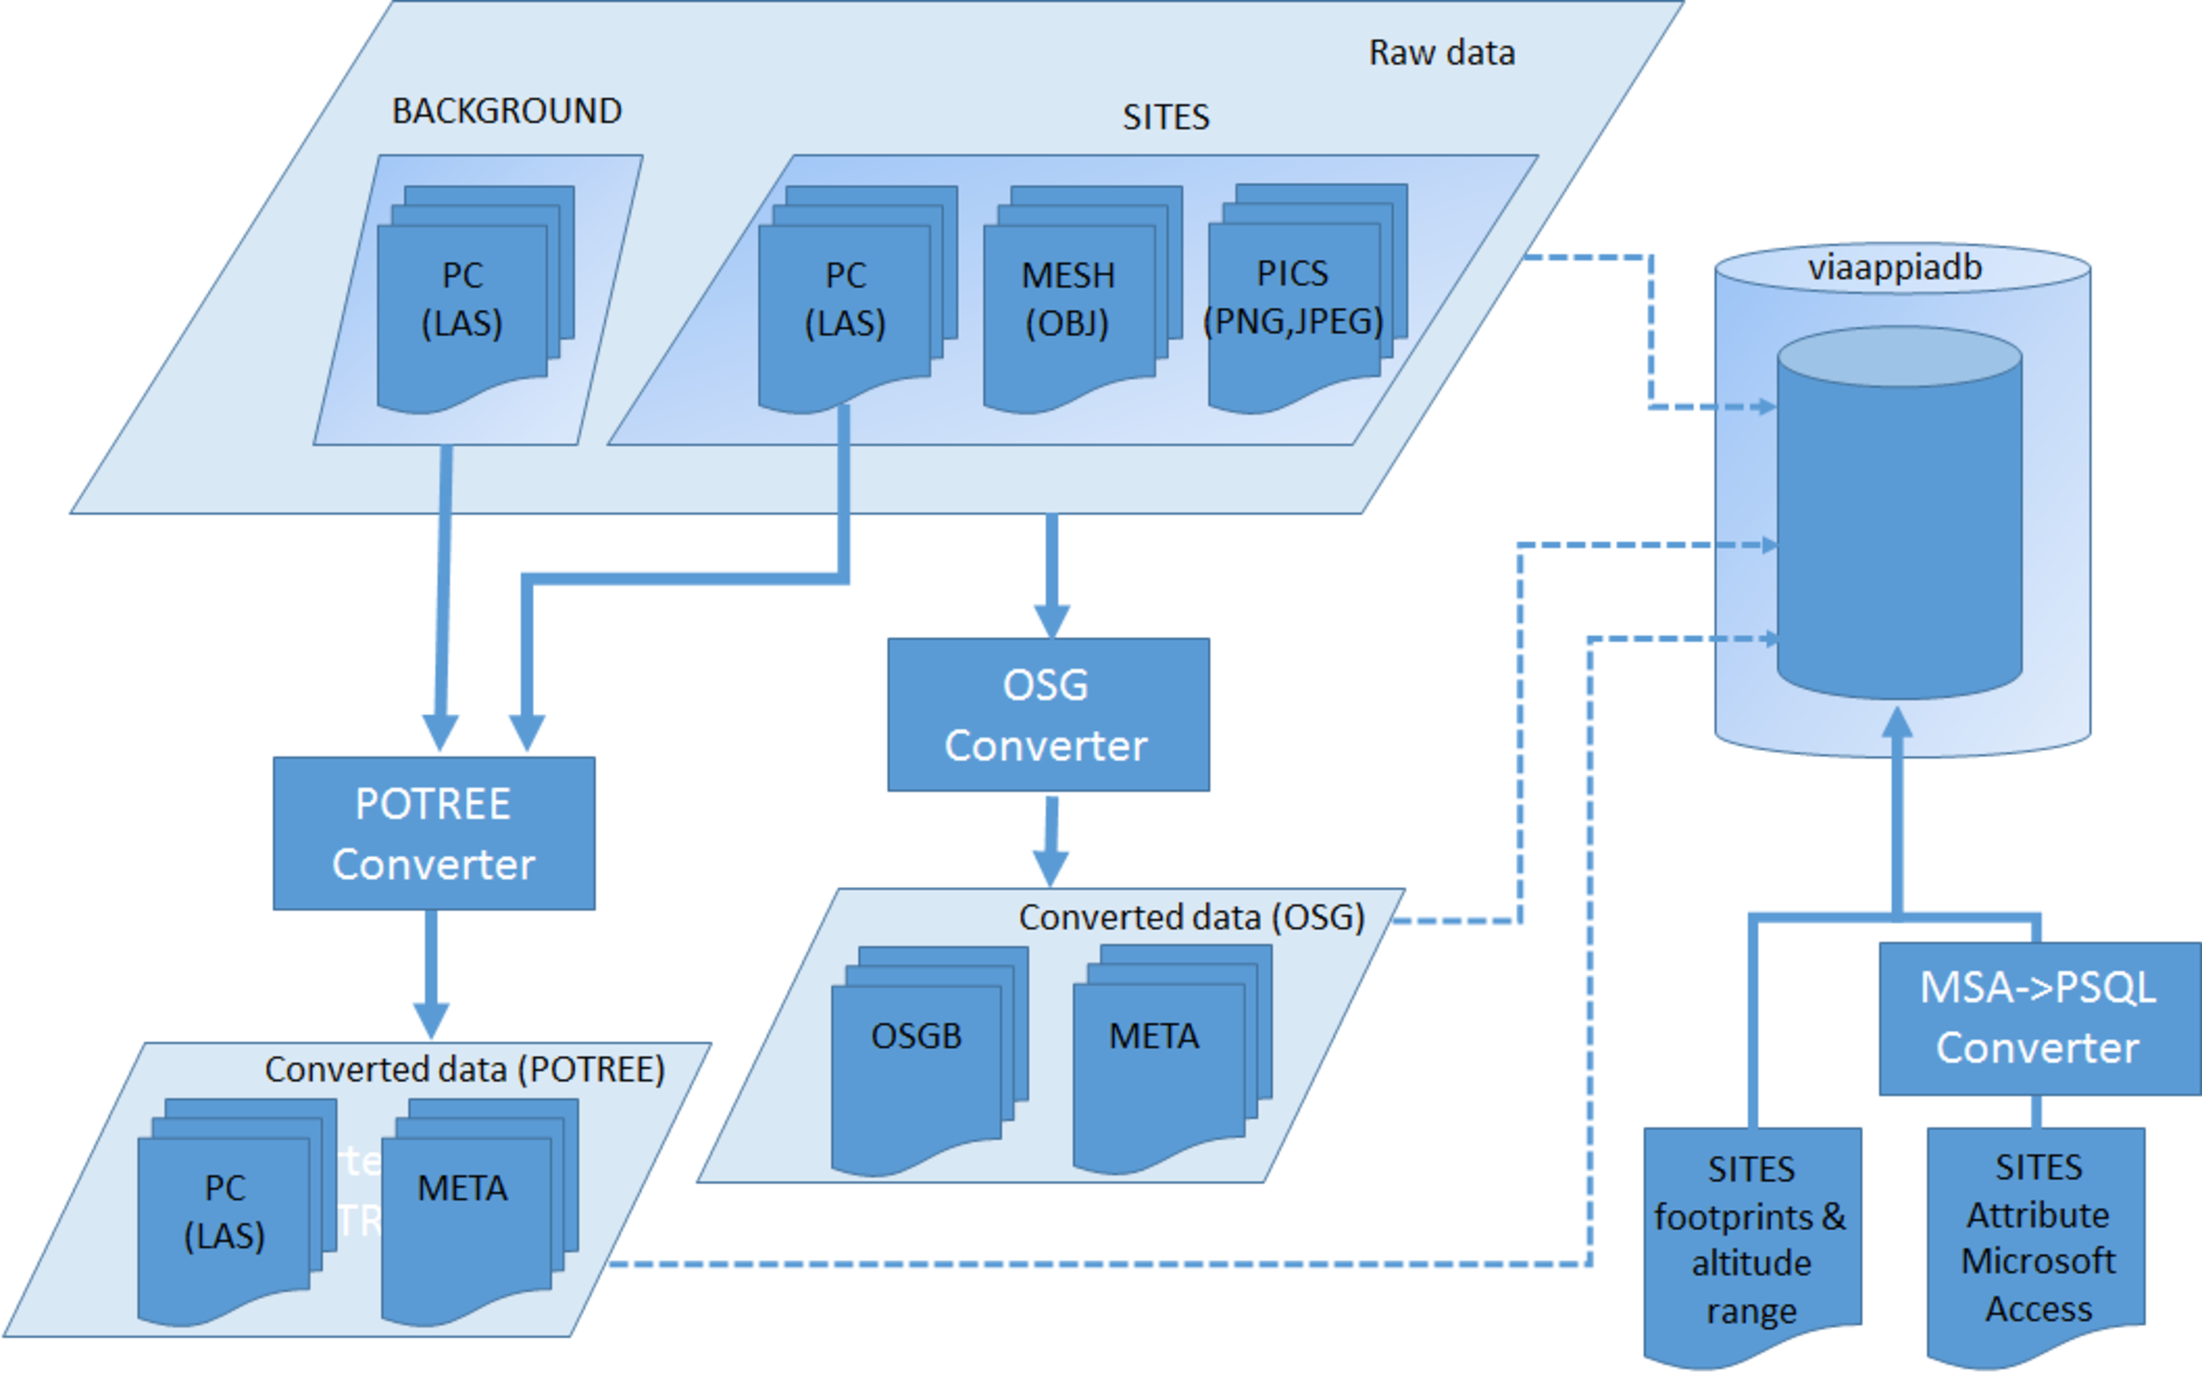
\includegraphics[width=0.75\textwidth]{fig/system_architecture/DataFramework.pdf}
 \caption{Data preparation framework executed on the Via Appia Linux serer}
 \label{fig:sys_arch_data_framework}
\end{figure}

Once the data preparation framework has been executed on the server the several clients can start using the 3D/4D GIS system. In the case of Windows desktops or laptops, local copies of the OSG  data required for visualization need to be downloaded. A \textit{launcher} tool based on the Xenon library (\url{http://nlesc.github.io/Xenon/}), developed by the Netherlands eScience Center (NLeSc), is used for this purpose. The tool also downloads the configuration file required by the 3D viewer. Once both the data and the configuration file are locally available in the client (Windows computer) the launcher tool automatically starts the 3D viewer. There is also a Web client which can use the POTREE converted point clouds. In this case no local copy of the data is needed for the 4D viewer, but the necessary data are pulled from the server on request via NGINX Web server (\url{nginx.com}). The viewer also needs a JSON configuration file containing the meta-data for the background and the sites obtained from the {\em viaappia} DB. The 4D viewer have been developed by NLeSc. Figure \ref{fig:sys_arch_2tier} illustrates the two-tier architecture and shows the steps performed at the client side. 

Both the execution of the data preparation framework in the server and the steps in the client have been automated. The user is referred to Section \ref{sec:software} for instruction of how to use the architecture.

\begin{figure}[H]
 \centering
 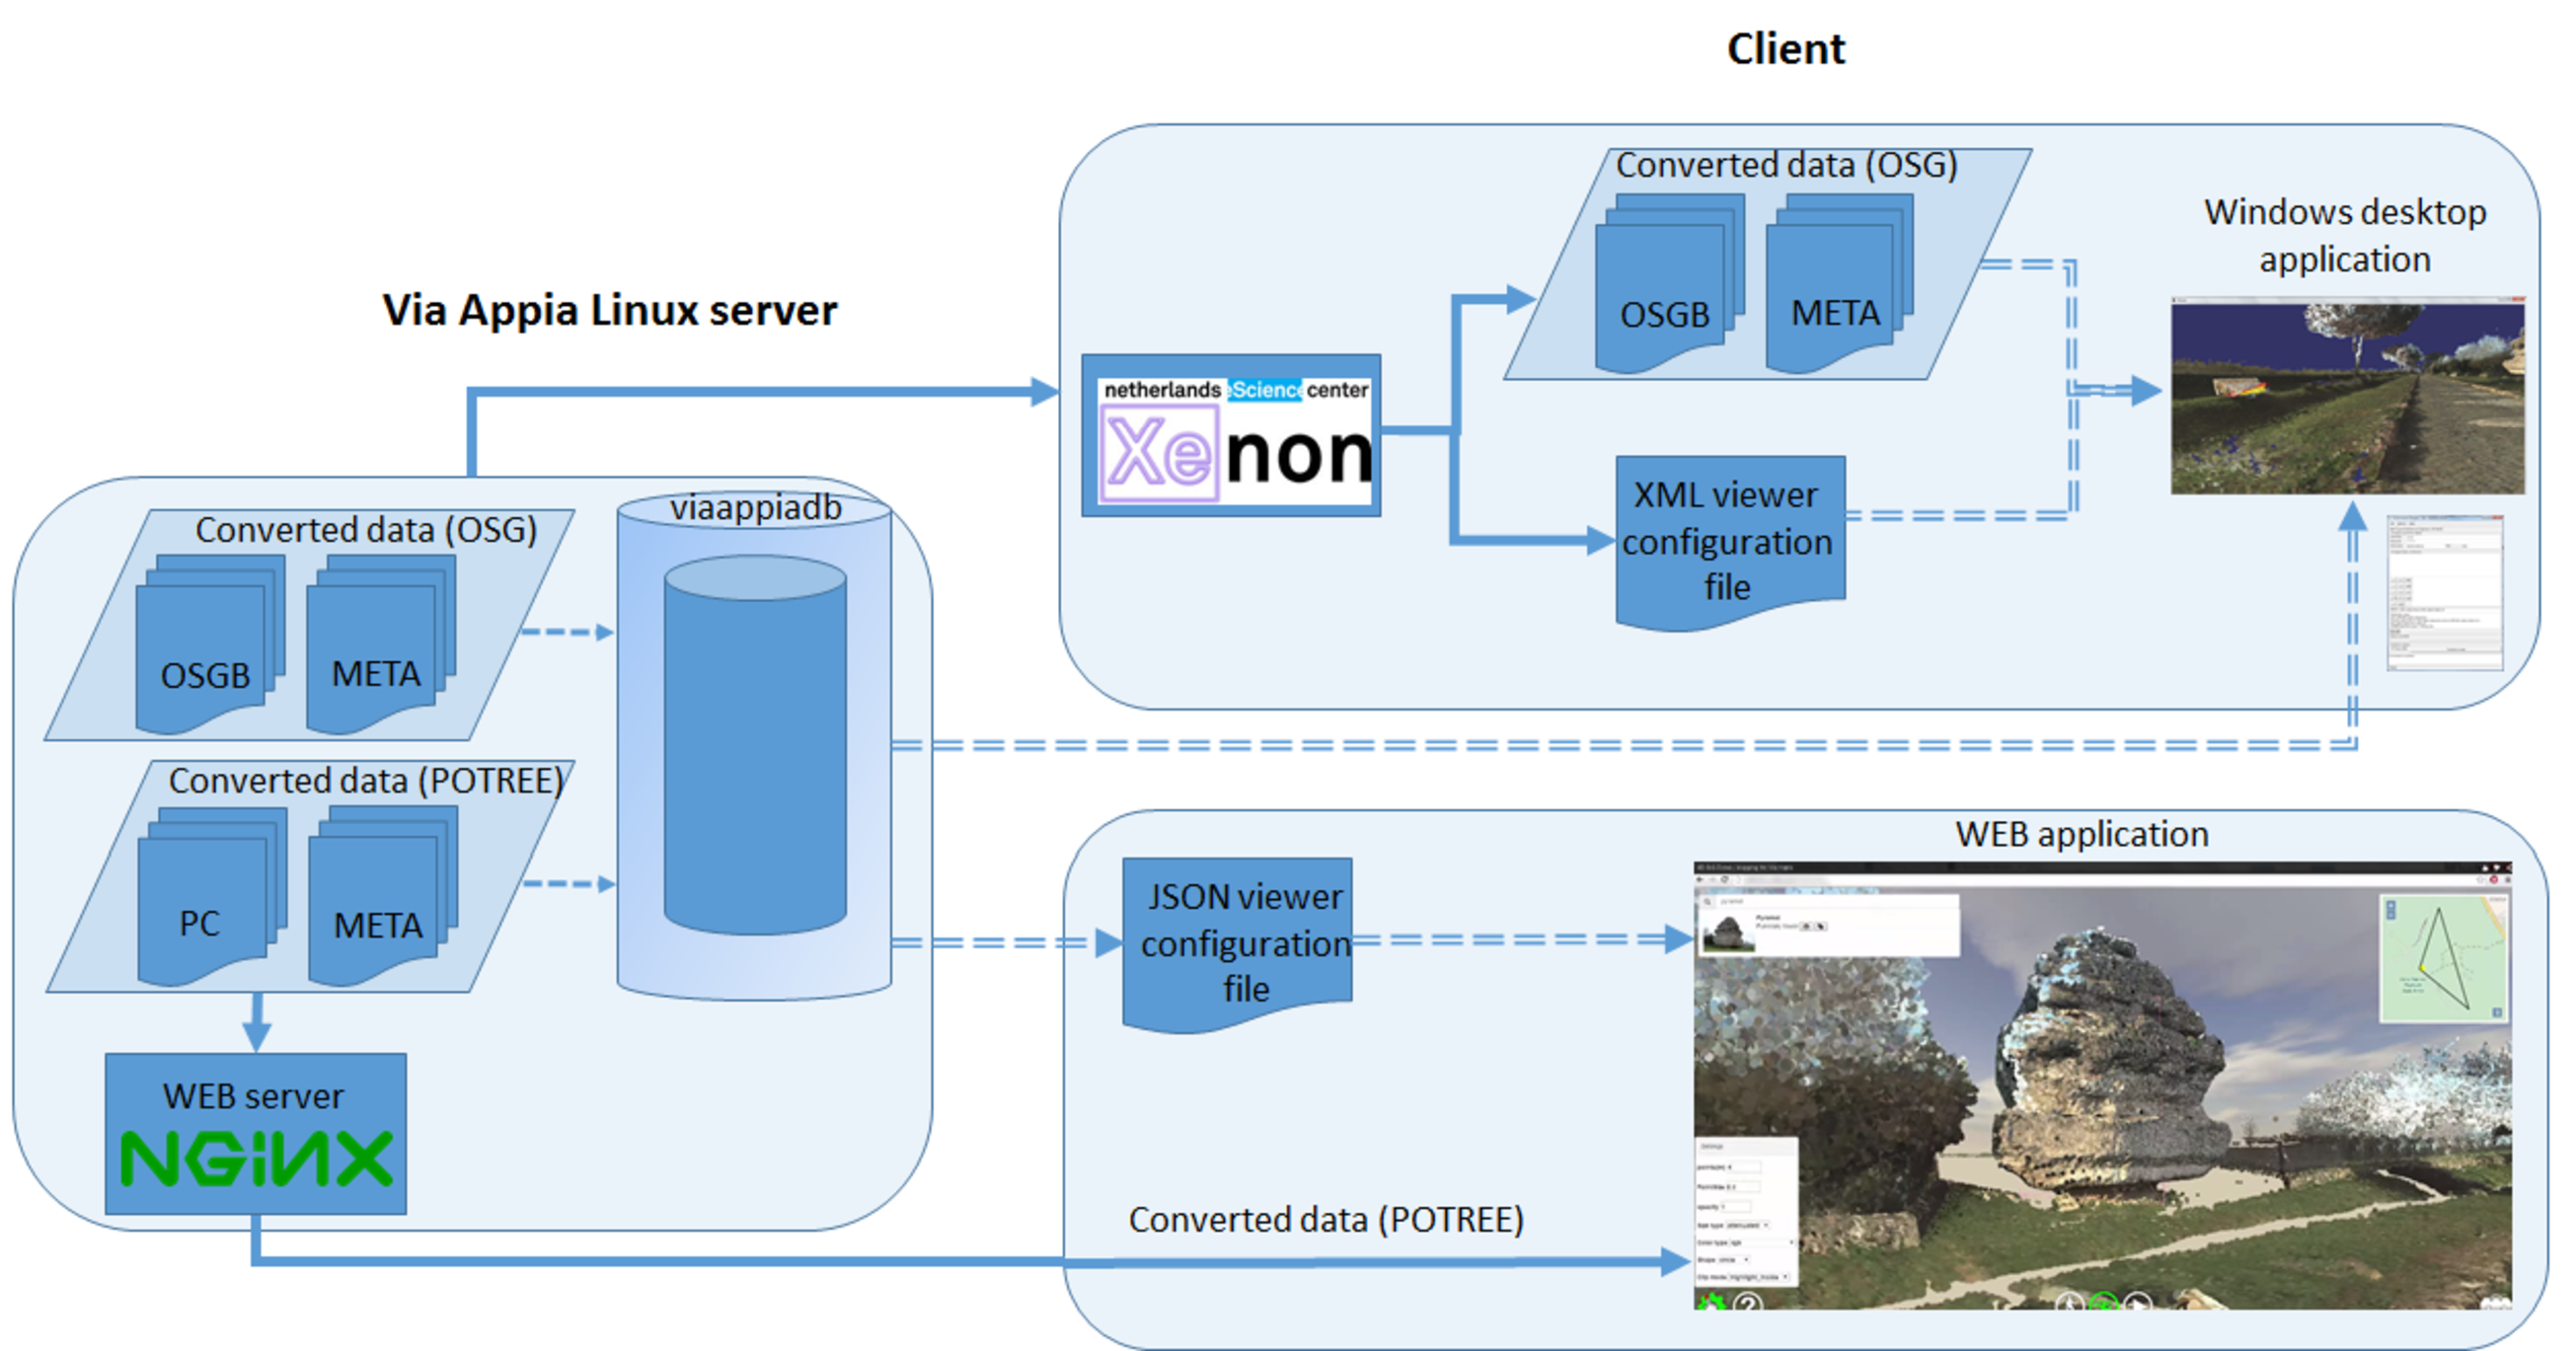
\includegraphics[width=0.95\textwidth]{fig/system_architecture/TwoTierArchitecture.pdf}
 \caption{Two-tier architecture of the Via Appia 3D/4D GIS and the steps executed on the client side.}
 \label{fig:sys_arch_2tier}
\end{figure}